\section{Query Implementation}
In this section, we elaborate how we have implemented the query logic to achieve O(log(n)) time complexity. The 2015 Grand Challenge problem has two queries. First is to evaluate top ten most frequent routes within last 30 minutes and second is to evaluate top ten profitable areas within last 15 minutes. We can use a composite object to keep route details for each route and fare details to each cell to compare values among routes and cells. However, each time window can have thousands of route and cell details. Therefore an efficient data structure is required to add, remove, update and retrieve top ten values from a set of objects for a given time window efficiently. Further since each event is received with route and cell details, above mentioned operations should perform using route and cell details as the key. In order to support all these functions with O(log(n)) time complexity we developed a data structure called NodeList. Following parts of this section describes how we have achieve this time complexity with \textit{NodeList} data structure and how we have implemented the queries using that data structure.

\subsection{NodeList data structure}

\begin{table}
\centering
\caption{Operations of \textit{NodeList} Data Structure}
\begin{tabular}{|l|l|} \hline
Operation Signature & Time Complexity \\ \hline \hline
add(key : Object, value : NodeValue) & O(log(n)) \\ \hline 
get(key : Object) : NodeValue & O(1) \\ \hline
remove(key : Object) : NodeValue & O(log(n)) \\ \hline
decrementPosition(key : Object) & O(log(n)) \\ \hline
incrementPosition(key : Object) & O(log(n)) \\ \hline
getTopValues() : List<NodeValue> & O(1) \\ \hline
\end{tabular}
\label{nodelist_api}
\end{table}

Table \ref{nodelist_api} shows the operations of this data structure. The NodeValue is an interface to plug any user defined type as a value. For an example, the route query can use a RouteCount object to keep route count while profitable cells query can use CellProfict object to keep fare details. This interface contains a method called compare to define the order of the values. The NodeList data structure provides the notion of a sorted values starting from position 0 (highest value) to its users. The decrementPostion operation moves the corresponding value towards position 0 until the correct position according to sorted order. Therefore this method should be called after increasing a value of an existing object. Similarly incrementPosition operation can be used to move a value to correct position after decreasing the value of an existing object. GetTopValues operation returns the top ten values of the list. Query algorithm sections further elaborate usage of these methods.

One way of implementing this data structure is to use a heap. Heap supports adding and extracting maximum value operations in O(log(n)) time. However since this application requires top 10 values, we need to retrieve maximum value ten times and insert them back, if we just a heap. On the other hand if we use a doubly linked list to keep values, it will take O(n) time for  decrementPostion and   incrementPosition operations. Therefore we can use a doubly linked list to keep first 10 values (this makes time complexity for all operations with this data structure O(1)) and heap to keep other values to avoid above problems.  A Map which points to values can be used to retrieve values using a key.

NodeList data structure uses two data structures called OrderedList to keep first 10 values and DynamicHeap to keep other values. In this way it has to change only the last value of OrderedList and maximum value of Dynamic heap as required. Following sections describes how these structures implemented with their operations.

\subsection{OrderedList data structure}

\begin{table}
\centering
\caption{Operations of \textit{OrderedList} Data Structure}
\begin{tabular}{|l|l|} \hline
Operation Signature & Time Complexity \\ \hline \hline
add(key : Object, value : NodeValue) & O(n) \\ \hline
containsKey(key : Object) : boolean & O(1) \\ \hline
get(key : Object) : NodeValue & O(1) \\ \hline
incrementPosition(key : Object) & O(n) \\ \hline
decrementPosition(key : Object) & O(n) \\ \hline
remove(key : Object) : NodeValue & O(1) \\ \hline
getLastPosition() : int & O(1) \\ \hline
getLastKey() : Object & O(1) \\ \hline
\end{tabular}
\label{orderedlist_api}
\end{table}

Table \ref{orderedlist_api} shows the operations of the \textit{OrderedList} data structure. First six methods has the same meanings as the \textit{NodeList} data structure and last two can be used to get the size of the list and the value of the last object. We internally keep a counter and a pointer to tail to support these operations in O(1) time. Figure \ref{orderedlist_impl} shows the implementation details. The Map structure (an HashMap) is used to retrieve object pointers with O(1) expected time. Each node of the doubly linked list points to previous and next nodes while storing the \textit{NodeValue}.


\begin{figure}[!t]
        \centering
        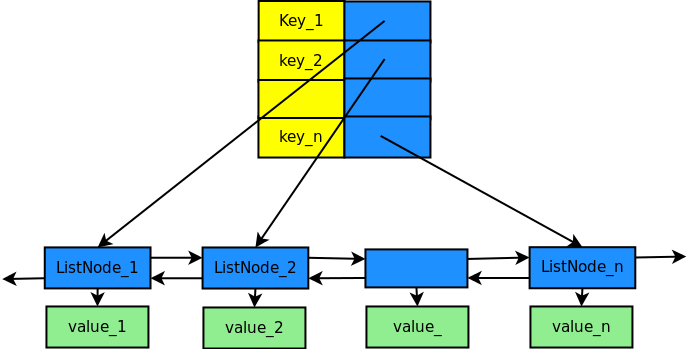
\includegraphics[width=3.0in]{orderedlist.png}
        \caption{\textit{OrderedList} data structure implementation}
        \label{orderedlist_impl}
\end{figure}
